\documentclass[11pt,french,professionalfonts]{beamer}

%\usefonttheme{serif}
%\usepackage{newpxtext,newpxmath}
\usepackage[utf8]{inputenc}
\usepackage[T1]{fontenc}
\usepackage{mathtools,amssymb,stmaryrd}

\SetSymbolFont{stmry}{bold}{U}{stmry}{m}{n}
\usepackage{babel}
\newcommand*{\retour}{\mathord{\leftarrow}}
\newcommand*{\gauche}{\mathord{\blacktriangleleft}}
\newcommand*{\droite}{\mathord{\blacktriangleright}}
\newcommand*{\entree}{\mathord{\blacksquare}}

\newcommand*{\suppr}{\mathord{\rightarrow}}
\newcommand{\egauche}[1]{\overleftarrow{\mathtt{#1}}}
\newcommand{\edroite}[1]{\overrightarrow{\mathtt{#1}}}


\newcommand*{\Clav}{\ensuremath{\mathsf{Clav}}}
\newcommand*{\Rat}{\ensuremath{\mathsf{Rat}}}
\newcommand*{\Rec}{\ensuremath{\mathsf{Rec}}}
\newcommand*{\Alg}{\ensuremath{\mathsf{Alg}}}
\newcommand*{\Cont}{\ensuremath{\mathsf{Cont}}}

\newcommand*{\MK}{\ensuremath{\mathsf{MK}}}

\newcommand*{\EK}{\ensuremath{\mathsf{EK}}}
\newcommand*{\RK}{\ensuremath{\mathsf{RK}}}
\newcommand*{\REK}{\ensuremath{\mathsf{REK}}}

\newcommand*{\FK}{\ensuremath{\mathsf{FK}}}
\newcommand*{\FEK}{\ensuremath{\mathsf{FEK}}}
\newcommand*{\FRK}{\ensuremath{\mathsf{FRK}}}

\newcommand*{\GK}{\ensuremath{\mathsf{GK}}}
\newcommand*{\GRK}{\ensuremath{\mathsf{GRK}}}
\newcommand*{\GEK}{\ensuremath{\mathsf{GEK}}}

\newcommand*{\FREK}{\ensuremath{\mathsf{FREK}}}
\newcommand*{\GREK}{\ensuremath{\mathsf{GREK}}}
\newcommand*{\BREK}{\ensuremath{\mathsf{BREK}}}

\newcommand*{\QMK}{\ensuremath{\mathsf{QMK}}}
\newcommand*{\QRK}{\ensuremath{\mathsf{QRK}}}
\newcommand*{\QGRK}{\ensuremath{\mathsf{QGRK}}}
\newcommand*{\QFRK}{\ensuremath{\mathsf{QFRK}}}

\newcommand*{\BK}{\ensuremath{\mathsf{BK}}}
\newcommand*{\BRK}{\ensuremath{\mathsf{BRK}}}

\let\touche\mathtt
\let\key\touche

\newcommand*{\conf}[2]{
	\left\langle #1 \middle| #2 \right\rangle
}
\let\config\conf


\newcommand*{\act}[1]{\xrightarrow{#1}}
\newcommand*{\actEff}[1]{\xrightarrow{#1}_{\text{e}}}
\newcommand*{\cdotEff}{\odot} %{\cdot_{\text{e}}}
\usetheme{metropolis}
\metroset{progressbar=frametitle}
\metroset{block=fill}

\usepackage{xcolor}

\usepackage{tikz}     % Un package pour les dessins
\usepackage{tikz-cd}
\usetikzlibrary{cd, automata,positioning,arrows}
\usepackage{adjustbox}

\renewcommand{\L}{\mathcal{L}}
\renewcommand{\bar}{\overline}
\newcommand{\A}{\mathcal{A}}
\newcommand{\Kinf}{||K||_{\infty}}


\title{Claviers symétriques et à états}
\author[Erwann LOULERGUE]{Erwann LOULERGUE, \texorpdfstring{\\supervisé par Vincent PENELLE et Corto MASCLE}{}}
\date{Juin \& Juillet 2022}
\institute[ENS Paris-Saclay]{Au LaBRI}


\begin{document}

\begin{frame}
	\titlepage
\end{frame}

\begin{frame}{Sommaire}
	\tableofcontents
\end{frame}

\section{Les claviers "habituels"}
\begin{frame}
	\frametitle{Le contexte}
	\begin{center}
		\includegraphics[height=0.3\textwidth]{Drame.jpg}	
	\end{center}

	On possède un clavier ne fonctionnant pas normalement. 

	Quels mots peut-on écrire avec ce clavier ? Et de manière générale, étant donné un clavier, peut-on écrire un mot donné ?

\end{frame}
\begin{frame}{Définitions}
	\begin{block}{Opérations élementaires}
		\begin{itemize}
			\item $\touche{a}$ pour $a \in \Sigma$: écrit "a" à gauche du curseur. \pause
			\item $\retour$: efface la lettre à gauche du curseur. \pause
			\item $\gauche$ et $\droite$: déplace le curseur à gauche ou à droite.
		\end{itemize}
	\end{block}
	\vspace{-8pt}
	On note $S$ l'ensemble des opérations élémentaires.
	\pause
	\begin{block}{Claviers}
		\begin{itemize}
			\item Une \emph{touche} est une suite d'opérations élémentaires. \pause
			\item Un \emph{clavier (automatique)} est un ensemble fini de touches.
		\end{itemize}
	\end{block}
	\begin{exampleblock}{Le clavier précédent}
		Par exemple, le clavier discuté précedemment est $\{\touche{abc},\retour^2\}$
	\end{exampleblock}
\end{frame}

\begin{frame}{Modélisation}
	Quand le mot courant est $uv$ avec le curseur entre $u$ et $v$, on note la configuration $\conf{u}{v}$. \pause

	Les opérations élémentaires induisent des actions sur les configurations :
	\begin{align*}
		\forall a \in A&, \conf{u}{v}\cdot a = \conf{ua}{v} \\
		\conf{\varepsilon}{v}\cdot \retour = \conf{\varepsilon}{v} &, \conf{ua}{v}\cdot \retour = \conf{u}{v} \\
		\conf{\varepsilon}{v}\cdot \gauche = \conf{\varepsilon}{v} &, \conf{ua}{v}\cdot \gauche = \conf{u}{av} \\
		\conf{u}{\varepsilon}\cdot \droite = \conf{u}{\varepsilon} &, \conf{u}{av}\cdot \droite = \conf{ua}{v} \\
	\end{align*}
\end{frame}

\begin{frame}{Modélisation}
	\begin{exampleblock}{Action d'une touche}
		On applique $t = \retour a \droite$ à $\config{c}{d}$. \pause
		 \begin{align*}
			\config{c}{d} & \act{\retour} \config{\varepsilon}{d}\\
						  & \act{a}       \config{a}{d}\\
						  & \act{\droite} \config{ad}{\varepsilon}.
		\end{align*}
		Ainsi $\conf{c}{d}\cdot t = \conf{ad}{\varepsilon}$.
	\end{exampleblock}
	
\end{frame}

\begin{frame}{Les \emph{vrais} claviers} 
	Ces claviers sont assez limités : on n'a pas de notion de saisie qu'on choisirait d'arrêter. \pause On définit donc les \emph{claviers manuels} :
    \begin{block}{Clavier (manuel)}
        Un clavier manuel, ou simplement \textbf{clavier}, est un couple $(T,F)$ d'ensembles finis de touches.
        Une exécution acceptante d'un clavier est une suite de touches de $T$ suivie d'une touche de $F$.
    \end{block} \pause
	\begin{exampleblock}{Remarque}
		Le fait qu'une touche soit finale peut être modélisé par une touche entrée qu'on notera $\entree$.
	\end{exampleblock}
\end{frame}

\begin{frame}{Le langage d'un clavier}
	Pour les claviers automatiques, on a \[\L(K) = \{w | w =uv, \exists t_1...t_n, \conf{\varepsilon}{\varepsilon}\cdot t_1...t_n = \conf{u}{v}\}\] \pause
    Sinon, dans le cas général, on définit $\L(K)$ comme \[\{w | w =uv, \exists t_1...t_n, \conf{\varepsilon}{\varepsilon}\cdot t_1...t_n = \conf{u}{v}, \mathrm{seule~} t_n \mathrm{~est~finale}\}\]
\end{frame}


\begin{frame}
	\frametitle{Classes de claviers}
	\[
	 \begin{array}{cc}
		\mathsf{R}:  \retour & \mathsf{E}:  \entree \\
        \mathsf{G}:  \gauche & \mathsf{F}:  \droite + \gauche \\
	 \end{array}
	\]

	\[
		\begin{array}{ccc}
			\MK : \{\} & \GK : \{\gauche\} & \FK :\{\gauche,\droite\} \\
			\EK : \{\entree\} & \GEK : \{\gauche,\entree\} & \FEK :\{\gauche,\droite,\entree\} \\
			\RK : \{\retour\} & \GRK : \{\gauche,\retour\} & \FRK :\{\gauche,\droite,\retour\} \\
			\color{orange}{\REK : \{\retour, \entree\}} & \GREK : \{\gauche,\retour,\entree\} & \FREK :\{\gauche,\droite,\retour,\entree\} \\
		\end{array}
	\]
	\small{Par abus de langage, on dira qu'un langage est dans une classe pour dire qu'il est reconnu par un clavier de cette classe.}
 \end{frame}


\section{Claviers à états}
\begin{frame}{Définition}
	\begin{block}{Clavier à état}
		Un clavier à états est la donnée de $(Q,\Delta ,F,s_0)$ où :
        \begin{itemize}
            \item $Q$ est un ensemble d'\textbf{états}
            \item $\Delta \subset Q \times S^* \times Q$\footnote{rappel : $S$ est l'ensemble des opérations élémentaires.} est un ensemble fini de \textbf{transitions}
            \item $F$ est un ensemble d'états dits \textbf{finaux}
            \item $s_0 \in Q$ est un état dit \textbf{initial}
        \end{itemize}
	\end{block}
	\pause
	\begin{block}{Configuration étatique}
		La configuration d'un clavier à états pendant son calcul est décrite par $(u,q,v) \in A^* \times Q \times A^*$, appelé \textbf{configuration étatique}.
	\end{block}
\end{frame}
\begin{frame}{Définition}
	\begin{exampleblock}{Action d'une touche sur une configuration}	
		Soit $(u,q,v)$ une configuration étatique, et $(q,t,q') \in \Delta$. En appliquant cette transition, on passe dans la configuration $(u',q',v')$, avec $\conf{u'}{v'} = \conf{u}{v} \cdot t$.
	\end{exampleblock}
	Une touche modifie le mot (clavier) et fait passer dans un autre état (automate).
	\pause
    On peut donc définir le langage d'un clavier à états :
    \[ \{uv | \exists\delta_1,...,\delta_n \in \Delta, \exists s_f \in F, (u,s_f,v) = (\varepsilon,s_0,\varepsilon)\cdot\delta_1\cdots\delta_n \}\]
	\pause
    On notera $\mathsf{Q}X$ l'ensemble des claviers à états dont les transitions sont toutes de classe $X$ : $\QMK$, $\QFRK$, \textit{etc}... 
\end{frame}
\begin{frame}{$\QRK = \Rat$}
	$\QRK$ est un bon candidat pour être égal à $\Rat$, car il ajoute des états à $\RK$.
	Une inclusion est triviale.
	\pause

	On veut donc montrer que pour tout clavier $K \in \QRK$, il existe un automate fini le simulant. Pendant un calcul, on regarde la structure de la zone de texte :
	
	\begin{figure}[!h]
		\centering


		\tikzset{every picture/.style={line width=0.75pt}} %set default line width to 0.75pt        

		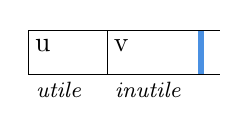
\begin{tikzpicture}[x=0.75pt,y=0.75pt,yscale=-1,xscale=1]
		%uncomment if require: \path (0,300); %set diagram left start at 0, and has height of 300
		
		%Straight Lines [id:da6237929847746642] 
		\draw    (100,115) -- (192.2,115) ;
		%Straight Lines [id:da44668726290788974] 
		\draw    (100,115) -- (100,136) ;
		%Straight Lines [id:da904664921210427] 
		\draw    (100,136) -- (192.2,136) ;
		%Straight Lines [id:da8679254388000219] 
		\draw    (138,115) -- (138,136) ;
		%Straight Lines [id:da3704878663207596] 
		\draw [color={rgb, 255:red, 74; green, 144; blue, 226 }  ,draw opacity=1 ][line width=2.25]    (183.2,115) -- (183.2,136) ;
		
		% Text Node
		\draw (102,118) node [anchor=north west][inner sep=0.75pt]   [align=left] {u};
		% Text Node
		\draw (140,118) node [anchor=north west][inner sep=0.75pt]   [align=left] {v};
		% Text Node
		\draw (102.5,138.5) node [anchor=north west][inner sep=0.75pt]   [align=left] {\textit{\footnotesize{utile}}};
		% Text Node
		\draw (140.5,138.5) node [anchor=north west][inner sep=0.75pt]   [align=left] {\textit{\footnotesize{inutile}}};
		
		
		\end{tikzpicture}
		
	  \end{figure}
\end{frame}
\begin{frame}{Le lemme clé}
	On va essayer de construire un automate $\A(K)$ dont les états seront $(s,k)$ pour $s$ un état de $K$, et $k$ la taille du suffixe inutile : l'automate lit une lettre quand $K$ écrit une lettre \emph{utile}.
	\pause

	\emph{A priori}, ces états ne sont pas en nombre fini\dots 
	\pause
	\begin{alertblock}{Lemme}
		Soit $K$ un clavier à états de $\QRK$. On peut borner le nombre de lettres inutiles nécessaires pour écrire tout mot de $\L(K)$ par un polynôme en $|K|$.
	\end{alertblock}
\end{frame}

\begin{frame}{La construction}
	\adjustbox{scale=0.6,center}{%
		$$
			\begin{tikzcd}[ampersand replacement=\&]
				{s_{\alpha,0}}                                                                                                                                     \&  \&  \& {s_{\beta,0}}              \&  \& {\overline{s_{\alpha,0}}} \arrow[rrrd, "\varepsilon", dashed]                                                                      \&  \&  \& \vdots                       \\
				\vdots                                                                                                                                             \&  \&  \& \vdots                     \&  \& \vdots                                                                                                                             \&  \&  \& {\overline{s_{\beta,|w|}}}   \\
				{s_{\alpha,r}} \arrow[rrruu, "w", bend left] \arrow[rrru, "{w[1,|w|-j]}", dotted] \arrow[rrr, "\dots", dotted] \arrow[rrrd, "\varepsilon", dashed] \&  \&  \& {}                         \&  \& {\overline{s_{\alpha,r}}} \arrow[rrru, "\varepsilon", dashed] \arrow[rrrdd, "w"] \arrow[rrrdddd, "{w[1]}"'] \arrow[rrrddd, dotted] \&  \&  \& {\overline{s_{\beta,|w|+1}}} \\
				{s_{\alpha,r+1}} \arrow[rrrd, "\varepsilon", dashed]                                                                                               \&  \&  \& {s_{\beta,|w|}}            \&  \& {\overline{s_{\alpha,r+1}}} \arrow[rrru, "\varepsilon", dashed]                                                                    \&  \&  \&                              \\
				\vdots \arrow[rrrd, "\varepsilon", dotted]                                                                                                         \&  \&  \& \vdots                     \&  \&                                                                                                                                    \&  \&  \& {s_{\beta,0}}                \\
				\vdots \arrow[rrrd, "\varepsilon", dotted]                                                                                                         \&  \&  \& \vdots                     \&  \&                                                                                                                                    \&  \&  \& {}                           \\
				{s_{\alpha,\mathcal{B}(K)}}                                                                                                                        \&  \&  \& {s_{\beta,\mathcal{B}(K)}} \&  \&                                                                                                                                    \&  \&  \& {s_{\beta,|w|-1}}           
			\end{tikzcd}
		$$
	}
	\begin{center}
		{\scriptsize Les transitions correspondantes à une touche $\alpha \xrightarrow{\retour^rw} \beta$}
		\pause

		Cet automate reconnaît le même langage que $K$.
	\end{center}
\end{frame}
\begin{frame}[standout]
	$\QRK = \Rat$
\end{frame}

\begin{frame}{Qu'a-t-on vraiment prouvé ?}
	Nous sommes partis des claviers de $\RK$, donc des machines qui écrivent et effacent, et nous leurs avons rajouté des états.
	\pause

    En prenant le point de vue opposé (en partant des automates), notre résultat peut se formuler comme ceci : \\
    \emph{Les automates pouvant effacer des lettres ont exactement la même expressivité que les automates habituels.}
\end{frame}

\section{Claviers symétriques}
\begin{frame}{Définition}
	\begin{block}{Opérations symétriques}
		Pour toute lettre $a \in A$, on définit les opérations d'écriture à gauche et à droite, $\egauche{a}$ et $\edroite{a}$, ainsi que l'effacement droit, noté $\suppr$.
        On définit leur sémantique :
        \begin{align*}
            \conf{u}{v} \cdot \egauche{a} &= \conf{ua}{v}   \\
            \conf{u}{v} \cdot \edroite{a} &= \conf{u}{av}   \\
            \conf{u}{av} \cdot \suppr &= \conf{u}{v}        \\
            \conf{u}{\varepsilon} \cdot \suppr &= \conf{u}{\varepsilon}
        \end{align*}
	\end{block} \pause
	On s'intéresse à $\BK$ $\left(\{\overleftarrow{A},\overrightarrow{A}\}\right)$ et $\BRK$ $\left(\{\overleftarrow{A},\overrightarrow{A},\retour,\suppr\}\right)$.

\end{frame}

\begin{frame}{Une structure inhabituelle}
	$\BK$ ne contient pas $\Rat$, et n'est pas contenu dedans non plus. 
	\pause

	Il n'est pas stable par union, et le caractère vide de l'intersection de deux langages de $\BK$ est indécidable.
	
\end{frame}

\begin{frame}{La conjecture principale}
	\begin{alertblock}{Conjecture}
		On suppose que $\BRK \subset \Alg$
	\end{alertblock}
	En effet, les principaux exemples de langages de $\BRK$ non rationnels sont $a^nb^n$ (langage de $\{\egauche{a}\edroite{b}\}$), ou bien les palindromes (langage de $\{\egauche{a}\edroite{a},\egauche{b}\edroite{b}, \dots\}$).
\end{frame}
\begin{frame}{La conjecture principale}
	\begin{alertblock}{Conjecture}
		On suppose que $\BRK \subset \Alg$
	\end{alertblock}
	Cependant, la méthode consistant à borner les lettres inutiles ne fonctionne pas, comme le montre le clavier $\{\egauche{a}\suppr,\retour\edroite{b}\}$.
\end{frame}

\begin{frame}[standout]
	Questions ?
\end{frame}
\end{document}